\chapter{Простейшая трехколесная тележка}
{\bfseries Анонс:}\\\\
Работа с блоком NXT и сервомоторами без компьютера. Использование разных элементов питания, заряд батареи на экране. Простейшая трехколесная тележка. Подача напряжений на моторы.
{\bfseries Цели:}
\begin{itemize}
	\item{}{\bfseries Обучающие:} Закрепить  основы работы в Lego Digital Designer. Ознакомить с основными типами элементов питания и их особенностями. Обучить программированию на блоке NXT.  
	\item{}{\bfseries Развивающие:} Сформировать умение прослеживать причинно-следственные связи.\\
\end{itemize}	
{\bfseries Ход занятия:}\\\\
\begin{tabular}{lll}
	\hyperlink{lesson4x1}{1. Организационный момент} & Презентация & (5 мин)\\
	\hyperlink{lesson4x2}{2. Батареи блока NXT} & Презентация & (20 мин) \\
	\hyperlink{lesson4x3}{3. Управление моторами} & Практика & (30 мин) \\
	\hyperlink{lesson4x4}{4. Простейшая трехколесная} тележка & Практика & (55 мин)\\
\end{tabular}\\\\

{\hypertarget{lesson4x1}{\blackBlueText{I.Организационный момент}}}\\\\

Первая часть сегодняшнего занятия посвящена работе с аккумуляторами и простейшему программированию блока NXT.Эта работа может выполняться фронтально, за партами.

Вторая часть занятия подразумевает самостоятельную работу в парах или по одиночке со свободным доступам к компьютерам, с установленным Lego Digital Designer и сохраненным на Рабочем столе файлом simple-car.lxf , и столам для конструирования.\\\\

{\hypertarget{lesson4x2}{\blackBlueText{II. Батареи блока NXT}}}\\\\

Несмотря на то, что чаще всего программа для робота сначала создается и редактируется на компьютере, а затем компилируется и загружается в память блока NXT, некоторые задачи можно решить, даже когда компьютера нет под рукой. 

Оговорим некоторые используемые ниже термины. {\bfseries Батарея}~--- это электрический компонент, обеспечивающий питание одного блока NXT. Батарея может состоять из нескольких элементов. {\bfseries Батарейка}~--- пальчиковый элемент питания не пригодный для перезарядки. {\bfseries Аккумулятор}~--- пальчиковый многократно перезаряжаемый элемент питания. 

Как уже говорилось, в качестве элементов питания можно использовать как фирменный аккумулятор Lego, так и пальчиковые аккумуляторы и батарейки размера АА.\\\\
\greenText{Картинка с вопросом}\\\\

Рассмотрим главные различия между последними двумя источниками, а также в процессе отметим основные отличия от фирменного блока питания. Большое преимущество аккумуляторов перед батарейками заключается в том, что разряженные аккумуляторы можно зарядить и снова ими пользоваться. Поэтому, несмотря на то, что аккумуляторы, как правило, дороже батареек (разница в цене примерно на порядок, а к этому нужно еще прибавить стоимость зарядного устройства), экономически их долгосрочное использование оказывается выгоднее. При этом только важно приобрести хорошее и качественное зарядное устройство, которое будет «лечить» аккумуляторы при каждом процессе заряда, не позволяя их емкости уменьшаться.

Что такое емкость аккумулятора? Фактически эта величина характеризует запас энергии, которую способен запасти аккумулятор, а потом в процессе работы ее отдать. Чем больше емкость, тем больше энергии запасает аккумулятор и тем дольше он будет ее отдавать~--- то есть дольше работать. Измеряется емкость в мАч (миллиампер*часы)~--- то есть, по сути, произведение тока на время его протекания. Так как батарейки или аккумуляторы соединяют последовательно (а при последовательном соединении ток во всех элементах цепи, как известно, один и тот же), то емкость батареи из последовательно соединенных элементов равна емкости одного элемента. Емкости современных батареек колеблются от 1500 до 3100 мАч, аккумуляторов от 1500 до 2700 мАч. Разумеется, имеет смысл приобретать элементы питания с наибольшей емкостью. Для сравнения, фирменный блок питания Lego (9693) имеет емкость 2100 мАч, проигрывая, таким образом, батарейкам и аккумуляторам большой емкости.

Кроме емкости есть еще один важный параметр~--- напряжение. Эта величина в нашем случае влияет на то, с какой скоростью аккумулятор будет отдавать накопленную у него энергию, то есть какую максимальную силу сможет развить робот в данные момент времени, или с какой максимальной скоростью он сможет двигаться. Если проводить сравнение с физиологией человека, то емкость~--- это выносливость (как долго человек будет справляться с нагрузкой), а напряжение~--- это мгновенная сила (может ли спортсмен сделать рывок, или поднять большой вес). Если несколько элементов питания соединить последовательно, то их напряжения складываются. Итак, напряжение одного стандартного аккумулятора 1,2 В, напряжение одной стандартной батарейки 1,5 В. Так как для питания блока NXT используется 6 элементов, то батарея из 6 аккумуляторов будет иметь напряжение 7,2 В, а батарея из 6 батареек – 9 В. Для сравнения, фирменный блок питания Lego (9693) имеет напряжение 7,4 В. В данном сравнении аккумуляторы значительно проигрывают батарейкам. Если посчитать аккуратно, то выдаваемая мощность батареек выше на 56 \%. 

Итак, какие выводы можно сделать на основе изложенных фактов?

{\slshape К этому моменту дети уже начинают терять внимание, поэтому прежде чем приступить к важным для нас выводам разумно выслушать их предположения, еще раз подчеркнуть какие-то моменты и вместе придти к следующему:}

{\bfseries Аккумуляторы выносливее батареек, но проигрывают им по мгновенной мощности.} Фирменная батарея Lego находится где-то посередине. В данной ситуации для повседневной работы выгодным является использование аккумуляторов,  батарейки же могут понадобиться в случаях, когда необходима большая мгновенная мощность – например, на соревнованиях.

{\slshape Еще один момент, который полезно знать, касается установки аккумуляторов. Внутри аккумуляторного отсека блока NXT есть небольшая черная кнопочка.}\\\\
\greenText{фото}\\\\

{\slshape При установке фирменного блока питания Lego эта кнопочка оказывается нажатой. Нажатие влияет на то, как блок NXT оценивает заряд блока аккумуляторов. Для правильной оценки кнопочка должна быть нажата. Таким образом, в некоторых ситуациях блок NXT неправильно отображает оставшийся заряд вставленных пальчиковых аккумуляторов или батареек. Блок NXT отображает значок состояния батареи в верхнем правом углу экрана.}\\\\
\greenText{Фото заряда батареи}\\\\

Рассмотрим теперь, на что влияет состояние батареи. Самое главное, и, пожалуй, единственное – на мгновенную мощность моторов (как следствие, на максимальную скорость их вращения). Не влияет на показания счетчиков оборотов моторов. Так как все датчики питаются стабилизированным напряжением 5 В, их показания также не зависят от состояния батареи.
Интересный момент: блок NXT перестает включаться, если напряжение батареи ниже 5 вольт.

По мнению автора, на момент издания настоящего пособия, оптимальным решением вопроса выбора элементов питания являются аккумуляторы GP NiMn R06 (AA) 2700 mAh в совокупности с зарядным устройством Ansmann ENERGY 16 (PLUS).

После того, как мы разобрались с питанием для блока NXT, мы можем наконец-то его включить.\\\\

{\hypertarget{lesson4x3}{\blackBlueText{III. Управление моторами}}}\\\\	

При включении блока NXT открывается главное меню на вкладке My Files. Нажав центральную оранжевую кнопку попадаем в раздел, где хранятся программы, загруженные с компьютера (Software files)  и написанные на NXT (NXT files). Кроме них там содержится папка Sound files, в которую автоматически сохраняются звуковые файлы из загруженных программ. Переходить между папками можно при помощи серых стрелок.\\\\
\greenText{рис}\\\\

Сегодня мы научимся писать простейшие программы на самом блоке. Для этого в главном меню переходим с вкладки My Files на вкладку NXT Program. Любая программа на NXT состоит из 5 блоков.\\\\
\greenText{Описание и пример программы.}\\\\

{\hypertarget{lesson4x4}{\blackBlueText{IV. Простейшая трехколесная тележка}}}\\\\	

Теперь соберем простейшую трехколесную тележку и запрограммируем ее на движение вперед. В качестве инструкции по сборке детям предлагается модель тележки, созданная в LDD. 

Что бы открыть файл выберем File\(\to\)Open. В появившемся окне выбираем путь, ведущий к искомому файлу.
\clearpage
\begin{figure}[h!]
	\begin{center}
		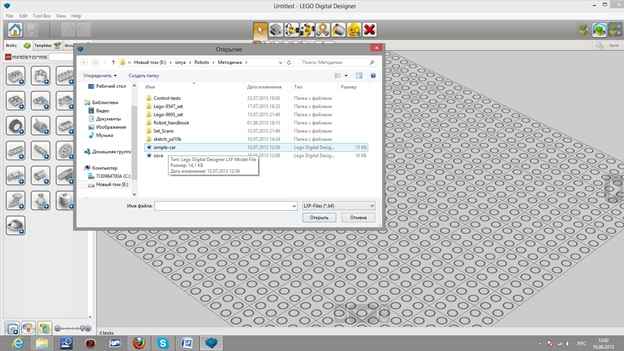
\includegraphics[width=0.95\linewidth]{chapters/chapter4/images/1}
		\caption{}
		\label{ris:image4x1}
	\end{center}
\end{figure}	 

Нажимаем «Открыть». Появляется модель тележки. Далее у детей есть свободное время (около 30 минут) на то, что бы собрать тележку в реальности. Методы которыми они при этом будут пользоваться не регламентированы~--- могу войти в режим «build guide», могут разбирать тележку по частым, могут просто крутить и приближать модель.

\begin{figure}[h!]
	\begin{center}
		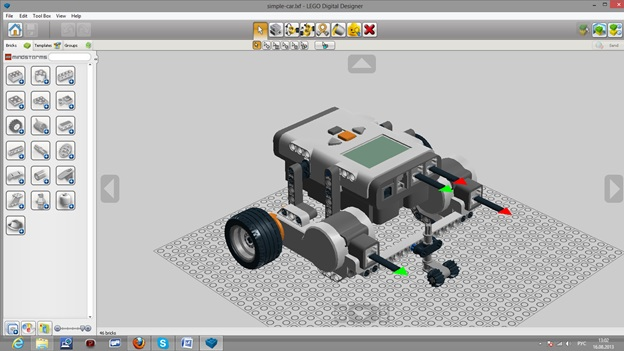
\includegraphics[width=0.95\linewidth]{chapters/chapter4/images/2}
		\caption{}
		\label{ris:image4x2}
	\end{center}
\end{figure}	

Итоговую тележку надо запрограммировать на блоке на движение прямо, как обсуждалось выше. Первый робот поехал!